\subsubsection{Sistema de Aireación }

Resulta indispensable conocer el momento de torsión necesario para mover la totalidad de la materia orgánica a procesar.

Una vez definido el tamaño del contenedor, es posible determinar la longitud máxima de las palas a utilizar.


\textbf{Cálculo de la fuerza generada}

El mecanismo de aireación estará encargado de la agitación de la materia orgánica al interior del contenedor, por lo que es importante determinar el peso total de la materia orgánica que será desplazada.

 Para la cantidad máxima de residuos que el compostador es capaz de procesar en cada lote, que es de 20 kilogramos, se tiene que el peso total es de:

  Por lo tanto:
\begin{center}
    $F = (20 Kg)(9.81 m/s^2)$ \\
    $F = 196.2 N $
\end{center}
Redondeando se obtiene:

 \begin{center}
     $F = 200 N $
 \end{center}




\textbf{Cálculo del Momento de torsión }

La fórmula del momento de torsión es:

\begin{center}
    $\tau=FdSin\theta$
\end{center}

Para el cálculo de la potencia requerida, se tomaron en cuenta la serie de valores siguientes, si el ángulo $\theta$ se considera máximo, al aplicar la carga con un ángulo de $90 ^o$ se tiene:

\begin{table}[h]
    \centering
    \caption{Datos críticos}
    \begin{tabular}{|c|c|}
        Parámetro & Valor \\
        \hline
        Peso de la materia orgánica & 200 N \\
        Longitud de las palas & 0.2 m 
    \end{tabular}
    \label{tab:DatosTor}
\end{table}

\begin{center}
    $\tau=(200 N)(0.2 m)(1)$ \\
    $\tau=40 Nm $
\end{center}



\textbf{Cálculo de la Potencia Consumida}

Para el cálculo de la potencia consumida para mover la materia orgánica es importante determinar la velocidad a la que girará el eje, así como el torque anteriormente calculado.

Al ser un sistema de baja velocidad constante de máximo 6 RPM, y si se sabe que:

\begin{center}
  $\omega = \frac{\theta}{t} $  
\end{center}
%Donde: \\
%$\theta$ son las vueltas en radianes \\
%$t$ es el tiempo en segundos
Se tiene entonces:
\begin{center}
    $\omega = \frac{(6 RPM)(2 \pi)}{60 s} rad/s$ \\
    $\omega = 0.6283 rad/s $ \\
    $\omega \approx 0.63 rad/s$
\end{center}

El cálculo de la potencia consumida se puede calcular con de la siguiente ecuación:

\begin{center}
 $P_{cons}=M_t * \omega$   
\end{center}

%Donde: \\

%$M_t$ es el Momento de torsión $\tau$ \\
%$\omega$ es la velocidad angular previamente calculada

Sustituyendo estos valores, se tiene que:
\begin{center}
    $P_{cons}=(40 Nm)(0.63 rad/s)$\\
    $P_{cons}=25.2 W$
\end{center}



\textbf{Selección del motor}

Una vez calculada la potencia consumida, por el eje de aireación es posible calcular y seleccionar el motor necesario para mover la carga.

Dado que se requiere una velocidad comprendida entre 3 y 6 rpm, y una potencia baja, el motor a seleccionar es un motor de baja potencia y baja velocidad.
$monofásico$

\begin{table}[h]
    \centering
    \caption{Características del motor seleccionado} 
    \begin{tabular}{c|c|c}
        Potencia & Tensión & RPM \\
        1/4 hp  & 127-220 V & 1750 
    \end{tabular}
    \label{tab:DatosMotro}
\end{table}

Se propone un reductor de velocidad conectado a la flecha del motor principal, el reductor se compone de una corona y un tornillo sin fin, ya que este mecanismo permite una alta relación de reducción.

La segunda etapa de reducción está compuesta por una banda de transmisión, ya que al ser un un mecanismo síncrono permite una velocidad constante a la salida, además de una eficiencia del $95\%$.

Al considerar las perdidas de potencia en las distintas etapas de reducción, se calculó la potencia real requerida. 

La eficiencia del reductor de corona y tornillo sin fin es de $82\%$.

Se tomará una eficiencia de $75\%$ para la caja reductora y $90\%$ para la banda.\cite{Mott}

\begin{center}
    $P_{Req}=\frac{(25.2 W)}{(0.75)(0.9)}$\\
\end{center}
\begin{center}    
    $P_{Req}=37.33 W\%$\\
\end{center}
\begin{center}
    $P_{Req}\approx 37.5 W\%$ 
\end{center}



\textbf{Diseño de la transmisión por Bandas}

Para realizar el diseño de la transmisión por banda, se requiere seguir la metodología mostrada en [cita],  la potencia requerida $(P_{req})$ debe ser multiplicado por un factor de servicio, dicho factor se muestra en la siguiente imagen
 (Figura \ref{fg:Factores}). 

De la tabla se observa que el factor de servicio para un motor eléctrico con movimiento uniforme es de 1.

Por lo que la potencia de diseño es igual a la potencia requerida.

\begin{center}
    $P_d = P_{req}=37.5 W$
\end{center}

Potencia de transmitida:  37.5 W=0.05 Hp \\
Velocidad entrada: 18 RPM $V_M=18 rpm$ \\
Velocidad salida: 5 RPM $V_C=5 rpm$ \\
Tiempo de uso:  < 6 horas por día \\


Se determinó el tipo de banda a utilizar con respecto a la siguiente imagen 
 (Figura \ref{fg:Bandas}). 

Se tiene una potencia y velocidad muy baja, por lo que la banda a  utilizar es 3VX.

La relación de velocidades nominales está determinada por:

\begin{center}
	$Relacion= \frac{18}{5} = 3.6$
\end{center}

Se calculó el tamaño de la polea motriz, si se desea tener una velocidad de la banda de $ v_b = 28 Ft/min$, como guía para seleccionar la polea motriz, el diámetro de la polea motriz está determinada por:
 
\begin{center}
	$D_M = \frac{18*v_b}{\pi*n_1}  =\frac{18*28}{\pi*18} = 8.91 in$
\end{center}

El tamaño de polea estándar más próximo es de:

\begin{center}
	$D_M = 9 in$
\end{center}

Para la polea conducida $P_C$ se buscó una que permita mantener la relación deseada

\begin{center}
	$D_C = \frac{9}{3.6 } = 2.5 in$
\end{center}

Revisando las tablas de valores estándar de las poleas se tiene:

\begin{center}
	$D_C = 2.5 in$
\end{center}

Se calculó la potencia nominal a partir de la tabla (\ref{fg:Banda3V}).

La potencia nominal de la banda es $P_n = 1 Hp$

Se calculó una distancia tentativa de la distancia de los centros utilizando la siguiente fórmula:

\begin{center}
	$ D_C < C < 3(D_C + D_M)$ \\
	$ 2.5 in < C < 3(2.5 + 9) in$ \\
	$ 2.5 in < C < 34.5 in $
\end{center}


Se propone una distancia $C$ de :

\begin{center}
	$C=17 in $
\end{center}

Se procedió a calcular la longitud de la banda necesaria, utilizando:
 
\begin{center}
	$L = 2C  + 1.57(D_C + D_M) + \frac{(D_C - D_M)^2}{4C}$ \\
\end{center}

Sustituyendo todos los valores se obtiene que:

\begin{center}
	$L =2(17) +1.57(9 + 2.5)+ \frac{(9 - 2.5)^2}{4(17)} = 52.68 in$
\end{center}

La longitud estándar más próxima al valor calculado, respecto a la tabla (\ref{fg:Longitud}).

Es de $L=53 in$ por lo que se procede a calcular la distancia real entre ejes, siguiendo la fórmula:

\begin{center}
	$B = 4L-6.28(D_C + D_M) = 4(53)-6.28(9 + 2.5) = 139.78$
	
\end{center}
	
\begin{center}
	$C = \frac{B+ \sqrt{(B)^2 - 32(D_C - D_M)^2}}{16} = \frac{139.78+ \sqrt{(139.78)^2 - 32(9 - 2.5)^2}}{16}$ \\
	$C=17.16 in$
\end{center}

Ahora se calculas el ángulo de contacto de la banda en la polea menor con la fórmula:

\begin{center}
	$\theta = 180^o - 2sen^{-1}[\frac{D_C - D_M}{2C}] = 180^o - 2sen^{-1}[\frac{9 - 2.5}{2*17.16}]= 177.34^o$
\end{center}

Determinar los factores de corrección con las tablas (\ref{fg:theta}) (\ref{fg:L}).

Por lo que se tiene que:

$C_\theta = 0.99$

Y para $L = 53 in$ en banda 3V $C_L = 0.96$  

La potencia normal corregida por la banda y la cantidad de banda necesarias para manejar la potencia de diseño.

\begin{center}
	$P_{correg} =C_\theta * C_L * P_N = 0.99 * 0.96 * 1/4 Hp$ \\
	$P_{correg} = 0.2376 Hp = 177 W$
\end{center}

Para determinar el número de bandas necesarias:

\begin{center}
	$N_B = \frac{P_d}{P_{correg}} = \frac{37.5 W}{177 W} = 0.21$ bandas 
\end{center}

Por lo que se utilizará 1 banda Tipo 3VX


\textbf{Diseño de la Cuña}

Para el diseño de la cuña se utiliza la norma ANSI B17.1-1967, la cual menciona que para ejes de hasta 6.5 pulgadas de diámetro, se utilizó una cuña cuadrada. Para determinar las dimensiones se utiliza la siguiente tabla:
 (Figura \ref{fg:Tamaños Cuña}). 

%\newpage

			
El tamaño de cuña para un eje de 1.5 pulgadas es de 3/8 pulgadas.

\begin{center}
	$W = \frac{3}{8} in = 9.52 mm$
\end{center}

El análisis para la cuña se realiza debido a las fallas potenciales que pueden tener al transmitir potencia, que son por corte y falla a la compresión.

Calculando la fuerza de tangencial $F_t$ que actúa sobre la cuña (Figura \ref{fg:Fuerza_T}). 

\begin{figure}[h]
    \centering
        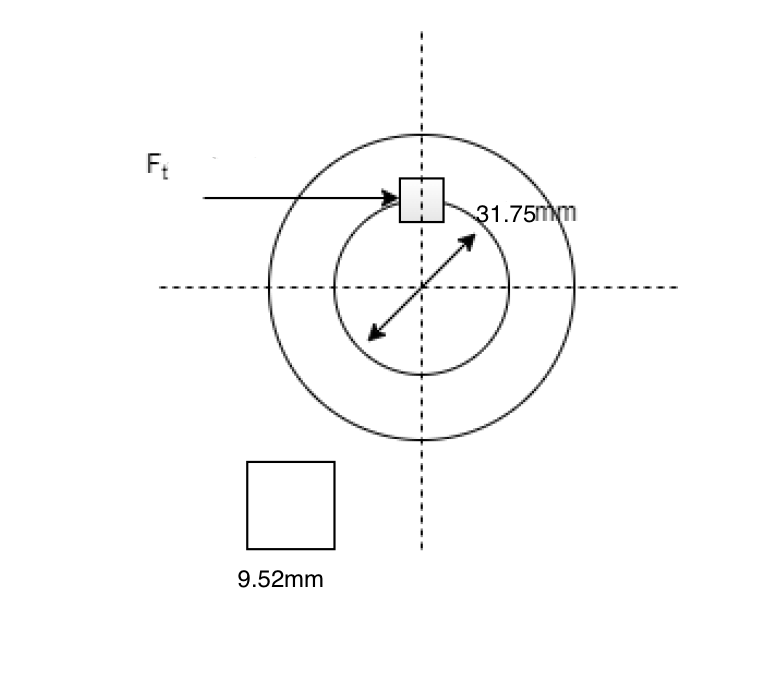
\includegraphics[scale=0.6]{images/Capitulo 4/s5/Fuerza Tangencia.png}
        \caption{Fuerza tangencial aplicada a la cuña}\cite{Mott}
    \label{fg:Fuerza_T}
\end{figure}
 

\begin{center}
	$F_t = \frac{2M_t}{d}$
\end{center}

Sustituyendo los valores previamente calculados, se tiene:

\begin{center}
	$F_t = \frac{2*40 Nm}{0.03175 m}$\\
	$F_t = 2519.68 N$\\
	$F_t \approx 2520 N$
\end{center}


En los diseños se puede igualar el esfuerzo cortante $S_y$ y el esfuerzo de diseño al cortante, para la teoría de falla por esfuerzo cortante máximo\cite{Mott}: 

\begin{center}
	$\tau_d = \frac{0.5*S_y}{N}$
\end{center}

Para aplicaciones industriales típicas, el libro \cite{Mott} recomienda $N=3$.

Si la cuña esta hecha del mismo material que el eje, acero SAE 1045, se tiene que:

\begin{center}
	$\tau_d = \frac{0.5*530.2 MPa}{3}$\\
	$\tau_d = 88.36 MPa$\\
	$\tau_d  \approx 88.5 MPa$
\end{center}

Si el esfuerzo cortante es:

\begin{center}
	$\tau = \frac{F}{A_s}$\\
	$\tau = \frac{F}{W*L}$
\end{center}

Para determinar la longitud mínima, por esfuerzo cortante, se despeja $L$ , por lo que se obtiene:

\begin{center}
	$L = \frac{F}{W*\tau}$\\
	$L = \frac{2520 N}{0.00952 m * 88.5 MPa}$\\
	$L = 2.98 mm$ \\
	$L \approx 3 mm$
\end{center}


Cálculo por aplastamiento:

\begin{center}
	$\sigma_d = \frac{\sigma_r}{N}$ \\
	$\sigma_d = \frac{630.2 MPa}{3}$ \\
	$\sigma_d \approx 210 MPa$
\end{center}

Sabiendo que el esfuerzo por aplastamiento es:

\begin{center}
	$\sigma = \frac{2*F}{H*L}$
\end{center}

Despejando $L$ se obtienes que: 
\begin{center}
	$L = \frac{2*F}{H*\sigma} = \frac{2*2520 N}{0.00952 m * 210 MPa}$
 \end{center}
 \begin{center}
	$L = 2.52 mm$ \\
	$L \approx 3 mm$
\end{center}

La cual es una longitud bastante pequeña, por lo que se propuso utilizar una con la longitud del ancho de la polea seleccionada. 


\textbf{Diseño del Eje de Aireación}

Para conocer las dimensiones reales del eje que se ve a utilizar el sistema de aireación, se usará la siguiente fórmula:

\begin{center}
    $D=\sqrt[3]{\frac{32*N}{\pi}*\sqrt{(K_t*\frac{M}{s'n})^2+ \frac{3}{4}*(\frac{T}{S_y})^2}}$
\end{center}

Se propone utilizar el acero ANSI 1045, porque es un acero de fácil adquisición, además de ser fácilmente maquinable,  tiene las siguientes características:

\begin{table}[h]
\begin{center}
\caption{Propiedades Acero ANSI 1045}
\begin{tabular}{| c | c | }
 \\ 
Característica & Magnitud \\ \hline
Dureza & $HB=179$  \\
Esfuerzo Máximo & $\sigma_r = 91.4 ksi$ \\
Esfuerzo de Fluencia & $S_y = 76.9 ksi$ \\
Elongación & $e=12\%$ \\ 
Reducción de área & $R_a=35\%$ \\ 
Maquinabilidad & $EF =55\%$ \\ 
    \end{tabular}
        \label{tab:A1045}
        \end{center}
\end{table}

El valor de la resistencia a la fatiga será vital a la hora de calcular el diámetro real de los ejes de transmisión, el cual se calcula:

\begin{center}
    $s'n =  sn*C_m*C_{st}*C_r*C_s$
\end{center}

El valor de sn se determina en función de la tabla siguiente (Figura \ref{fg:Res_fat}). 

De la gráfica se puede determinar que el valor a la fatiga teórico es de:

\begin{center}
    $sn=25 ksi$
\end{center}

Se sugiere un factor de material \cite{Mott}:
$C_m= 1$

Y un factor de esfuerzos:
$C_{st}=1$

Para determinar el Factor de confiabilidad se utiliza la siguiente tabla (Figura \ref{fg:Fac}). 

\begin{figure}[h]
    \centering
        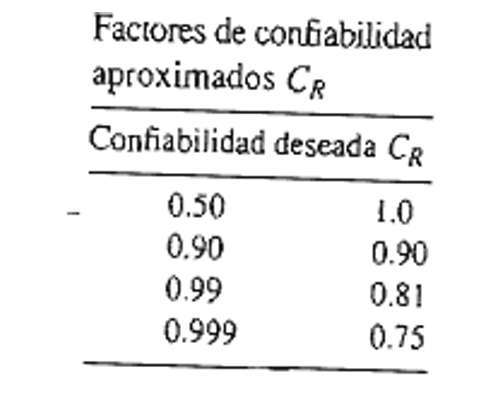
\includegraphics[scale=0.6]{images/Capitulo 4/s5/Factores de confiabilidad.png}
        \caption{Factores de confiabilidad}\cite{Mott}
    \label{fg:Fac}
\end{figure}

Se selecciona un grado de fiabilidad de 0.99, por lo que:

$C_r := 0.81$

Finalmente, para determinar el factor de tamaño se debe estimar el tamaño del eje, en función de la siguiente tabla (Figura \ref{fg:diseño}). 

\begin{figure}[h]
    \centering
        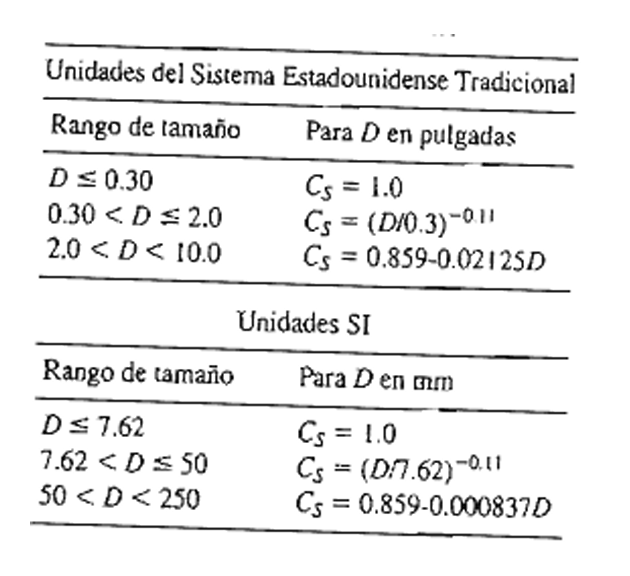
\includegraphics[scale=0.6]{images/Capitulo 4/s5/Factores de diseno aproximado.png}
        \caption{Factores de dise\~{n}o aproximado}\cite{Mott}
    \label{fg:diseño}
\end{figure}

Se estima que el eje tendrá un diámetro entre $0.3 in < D < 2.0 in $, se propone un valor máximo de 2 in. 

\begin{center}
    $D_{max}= 2 in$
\end{center}

Por lo que el factor de tamaño $C_s$ es:

\begin{center}
    $C_s = (\frac{D_{max}}{0.3})^{-0.11} = 0.812 $
\end{center}

Teniendo en cuenta todos estos factores, se procede a a reemplazar los en la fórmula de la resistencia de la fatiga real:

\begin{center}
    $s'n =  25 ksi*(1)*(1)*(0.81)*(0.812) = 16.44 ksi $
\end{center}

Ya determinado el factor de fatiga real, se procede a determinar las fuerzas que actúan sobre el eje, sabiendo que tendrá 3 palas y estarán 2 de un lado y una del otro, se tiene:

1 Pala(Figura \ref{fg:1pala}). 

\begin{figure}[h]
    \centering
        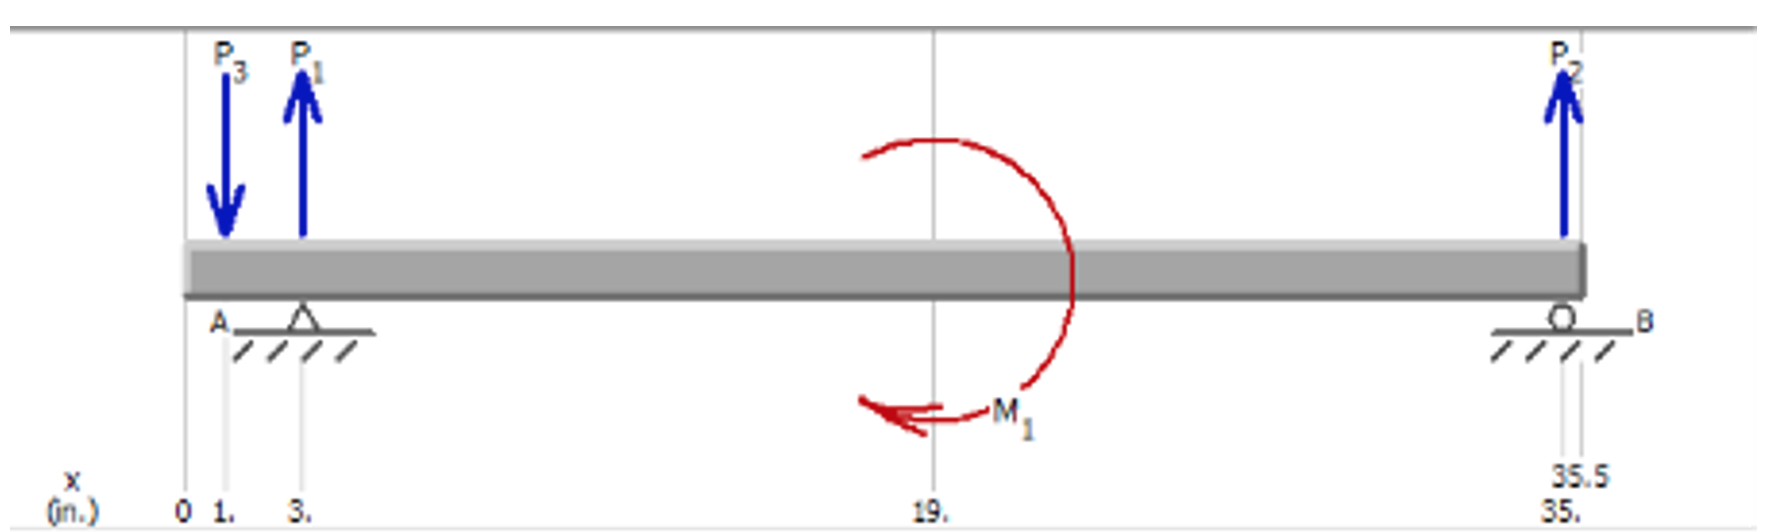
\includegraphics[scale=0.4]{images/Capitulo 4/s5/1 pala.png}
        \caption{Fuerzas del lado del eje con 1 pala}
    \label{fg:1pala}
\end{figure}

2 Palas(Figura \ref{fg:2palas}). 

\begin{figure}[h]
    \centering
        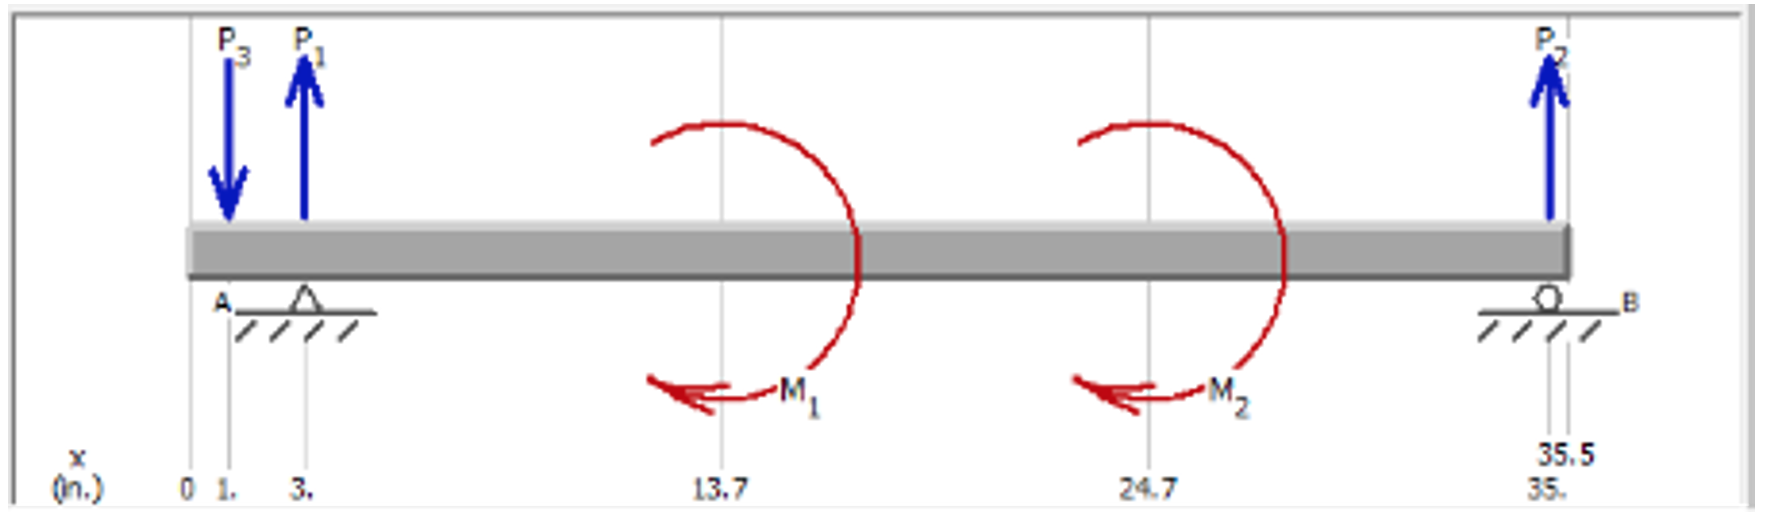
\includegraphics[scale=0.4]{images/Capitulo 4/s5/2 palas.png}
        \caption{Fuerzas del lado del eje con 2 palas}
    \label{fg:2palas}
\end{figure}

Donde: \\
P1 y P2 son las reacciones de la barra a su soportes. \\
P3 es la fuerza generada por la tensión de la banda 3V. \\
M1 con una pala y M1 y M2 representan el momento de torsión generado por las palas al instante de hacer girar la materia orgánica. \\ 

Para determinar  la fuerza generada por la tensión de la banda P3, se tiene:
\begin{center}
    $F_c = \frac{2T}{D}$
\end{center}

Donde: \\
T: es el torque al que se somete la polea \\
D: es e diámetro máximo de la polea \\

Si se tiene que:

\begin{center}
    $ T = 40 Nm$ \\
    $D_{polea}=2.5 in = 0.0635 m$
\end{center}

Entonces se tiene que la fuerza $F_c$ es:

\begin{center}
    $F_c = \frac{2*40 Nm}{0.0635m} = 1259.84 N $
\end{center}

Por lo que los diagramas de fuerzas quedan de la siguiente manera:

%\newpage
1 Pala(Figura \ref{fg:1palaF}). 

%\newpage 
2 Palas(Figura \ref{fg:2palasF}). 

Como se busca tener un eje de diámetro constante se toma el momento flexionante más grande de las gráficas, por lo que:

\begin{center}
    $M= 47.76 Nm$
\end{center}

Se define $K_t = 2.5$ de acuerdo a los valores propuestos para perfiles redondeados \cite{Mott}.

Y se selecciona un factor de seguridad $N=3$.

Con los datos obtenidos se procede a calcular el diámetro mínimo para el eje de transmisión,  sustituyendo todos los valores anteriores se tiene que:

\begin{center}
    $D=\sqrt[3]{\frac{32*3}{\pi}*\sqrt{(2.5*\frac{47.76 Nm}{16.64 ksi})^2+ \frac{3}{4}*(\frac{40 Nm}{76.9ksi})^2}} = 1.25 in$
\end{center}

Se puede ver que el diámetro mínimo de diseño es de $D=1.25 in$, sin embargo al ser el mínimo teórico calculado y no tomar en cuenta el posicionamiento del los rodamientos y las perforaciones que se le harán para poder sujetar las palas de agitación, se decidió seleccionar un diámetro $D=1.5 in$.

Esta medida permite mantener un diámetro efectivo de 1.25 pulgadas, a su vez colocar los rodamientos en su posición fácilmente.

Con estos datos calculados, se procedió a diseñar el siguiente eje de transmisión (Figura \ref{fg:eje}). 

\begin{figure}[h]
    \centering
        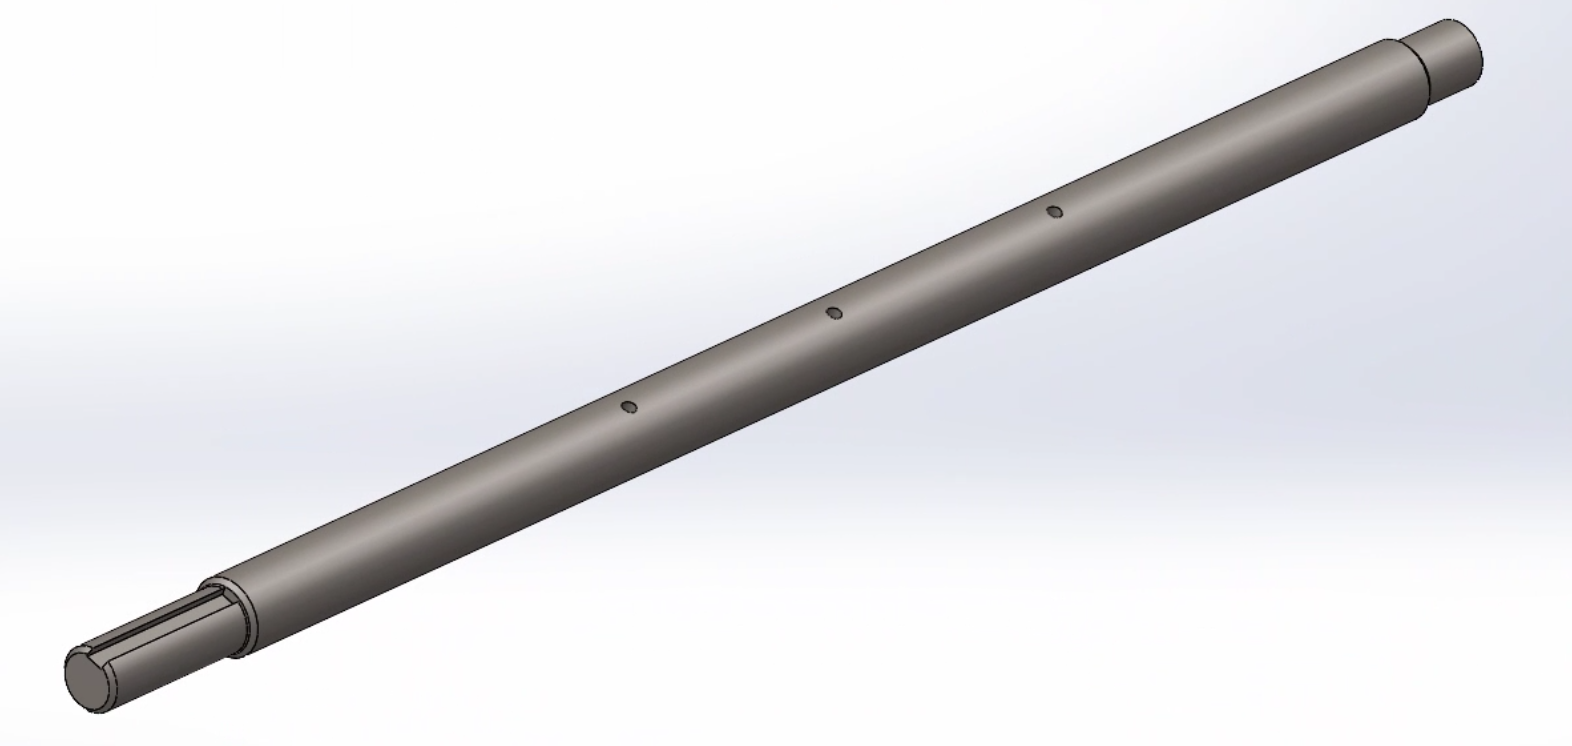
\includegraphics[scale=0.45]{images/Capitulo 4/s5/Eje Trituracion.png}
        \caption{Diseño de eje}
    \label{fg:eje}
\end{figure}


\newpage

\textbf{Validación del Eje.}

Para validar las dimensiones calculadas se procedió a hacer una simulación de estudio estático en SolidWorks.

Para ello se toma en consideración los puntos fijos, que representan lo rodamientos de apoyo, así como la fuerza ejercida por La banda de transmisión, además del par torsor al que esta sometido a lo largo del eje.

Para un estudio de esfuerzos aplicando el criterio de Von Mises (Figura \ref{fg:Esfuerzos}). 

\begin{figure}[h]
    \centering
        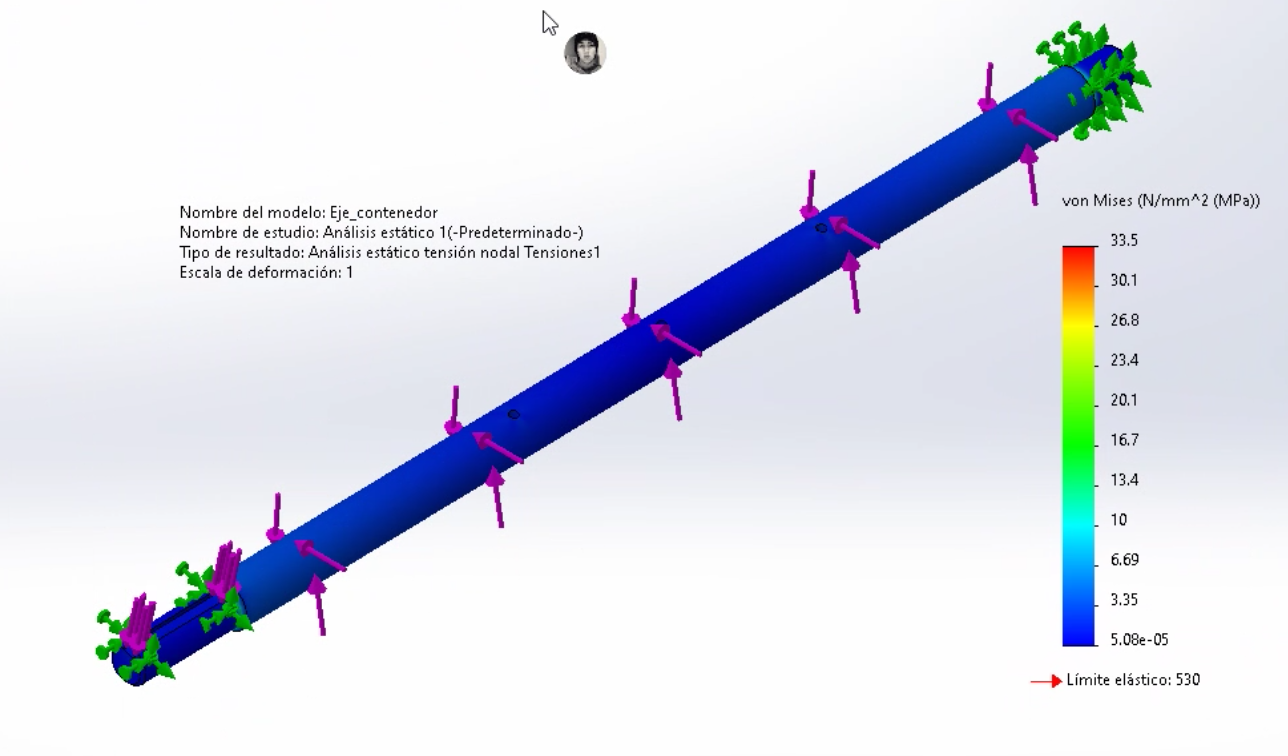
\includegraphics[scale=0.5]{images/Capitulo 4/s5/S5 validacion/Estudio Esfuerzos.png}
        \caption{Estudio Esfuerzos}
    \label{fg:Esfuerzos}
\end{figure}

Porque de la gráfica se observar que no existen puntos críticos en el eje, por lo que el eje no sufre riesgos de ruptura.